%!TEX TS-program = xelatex

%%%%%%%%%%%%%%%%%%%%%%%%%%%%%%%%%%%%%%%%%%%%%%%%
% CV template
% Originally created by Adrien Friggeri
% Improved by Carmine Benedetto
%%%%%%%%%%%%%%%%%%%%%%%%%%%%%%%%%%%%%%%%%%%%%%%%

\documentclass[]{cv-class}
\usepackage{afterpage}
\usepackage{hyperref}
\usepackage{color}
\usepackage{xcolor}
\hypersetup{
    colorlinks=true,
    linkcolor=blue
}
\RequirePackage{xcolor}
\definecolor{pblue}{HTML}{0395DE}

\begin{document}
\header{Martin}{Othamar}
      {full-stack developer}

% Fake text to add separator
\vspace{1.15cm}
\fcolorbox{white}{gray}{\parbox{\dimexpr\textwidth-2\fboxsep-2\fboxrule}{%
.....
}}

% In the aside, each new line forces a line break
\begin{aside}
  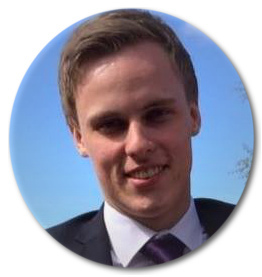
\includegraphics[scale=0.40]{img/meg2.jpg}
    ~
  \vspace{0.65cm}
  \section{Civil status}
    Married
  	~
  \section{Address}
    Trollkleiva 8\\
    4638 Kristiansand S\\
    Norway
    ~
  \section{Phone}
    +47 47 35 60 90
    ~
  \section{Mail}
    \underline{\href{mailto:martin@othamar.net}{martin@othamar.net}}
    ~
  \section{Web}
  	%\underline{\href{http://martinothamar.github.io}{martinothamar.github.io}}
	\vspace{0.10cm}
    \underline{\href{https://no.linkedin.com/in/martinothamar}{linkedin.com/in/martinothamar}}
	\vspace{0.10cm}
    \underline{\href{https://stackoverflow.com/story/martinothamar}{stackoverflow.com/story}}
	\vspace{0.10cm}
    \underline{\href{https://stackoverflow.com/cv/martinothamar}{stackoverflow.com/cv}}
	\vspace{0.10cm}
    \underline{\href{https://github.com/martinothamar}{github.com/martinothamar}}
    ~
  \section{Programming}
    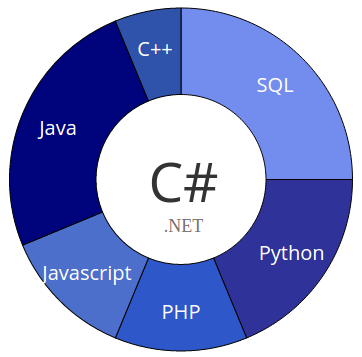
\includegraphics[scale=0.22]{img/programming.png}
    ~
  \section{OS Preference}
    \asidelist{\textbf{mac OS}}
    {
\includegraphics[scale=0.30]{img/star.png}
    
\includegraphics[scale=0.30]{img/star.png}
    
\includegraphics[scale=0.30]{img/star.png}
    
\includegraphics[scale=0.30]{img/star.png}
    
\includegraphics[scale=0.30]{img/star.png}}
    \asidelist{\textbf{Linux}}
    {
\includegraphics[scale=0.30]{img/star.png}
    
\includegraphics[scale=0.30]{img/star.png}
    
\includegraphics[scale=0.30]{img/star.png}
    
\includegraphics[scale=0.30]{img/star.png}
    
\includegraphics[scale=0.30]{img/star_empty.png}}
    \asidelist{\textbf{Windows}}
    {
\includegraphics[scale=0.30]{img/star.png}
    
\includegraphics[scale=0.30]{img/star.png}
    
\includegraphics[scale=0.30]{img/star.png}
    
\includegraphics[scale=0.30]{img/star_empty.png}
    
\includegraphics[scale=0.30]{img/star_empty.png}}
    ~
\end{aside}

\vspace{0.75cm}
\section{Experience}
\begin{entrylist}
  \entry
    {Nov. 15 - Now}
    {System Developer, Web}
    {Inkrement AS, Kristiansand}
    {Developing ed-tech related web \& mobile applications on stacks typically involving .NET C\# MVC/Web API on the back end
    and Razor/HTML/CSS/JS on the front end, and mobile development on native Android with Java.\\\\
    Wrote the ASP.NET Web API, SQLServer backend, including a React + Redux CMS front end and the native Android
    application for Eksamensklar (\underline{\href{http://erduklar.no/}{erduklar.no}}),
    a math exam preparation app for 10th graders in Norway.\\\\
    Worked on various pieces of the Campus Inkrement 
    (\underline{\href{https://campus.inkrement.no}{campus.inkrement.no}})
    flipped learning platform including the front
    page, initial infrastructure and administration for the Pro/Premium model, exception/error tracking system for the front and
    back end, as well as a Google Analytics reporting component allowing us better insight into usage patterns across the
    platform.\\}
  \entry
    {Sept. 15 - Now}
    {Co-Founder \& IT Consultant}
    {EnterCon AS, Kristiansand/Oslo}
    {A small consulting company delivering software-solutions, typically web \& mobile apps, software design, 
    development and marketing and innovation consulting.\\
	Developed and managed projects delivering web-apps, servers and mobile applications in both native 
	(iOS with Swift \& Android with Java) and hybrid formats (e.g. Ionic + Cordova + Meteor). \\}
  \entry
    {Aug. 15 - Nov. 15}
    {Software Developer}
    {meQuire Solutions AS, Kristiansand}
    {Part time back end development on a software-stack consisting of the following
    technologies; NodeJS, HAPI, RethinkDB.\\}
  \entry
    {Aug. 15 - Dec. 15}
    {Teaching Assistant}
    {University of Agder, Kristiansand}
    {Helping third year students in the IT and Information Systems Bachelor's degree programme
    learn in IS-213: Open Source Development.\\}
  \entry
    {Jan. 15 - May 15}
    {Bachelor thesis - IS-304}
    {Frontica Business Solutions, Kristiansand}
    {Full stack development and full remake/modernization of legacy Information Quality system
    on the .NET platform with C\# with technologies like ASP.NET Web Api 2,
    MVC, Windows Service, WCF,
    Twitter Bootstrap front end with JS/jQuery. Worked agile with Scrum on TFS 2012 /w TFVC
    and BDD for testing.
    \emph{Title of the Thesis:
    "The Reengineering of Frontica Business Solutions' Information Quality System".}
    Grade: \textbf{A}.\\}
  \entry
    {Sept. 14 - Dec. 14}
    {Internship - IS-302}
    {Frontica Business Solutions, Kristiansand}
    {Documentation of in-house VBA application as well as full stack development of
    in-house Active Directory
    user information reporting service on the .NET platform with C\#. ASP.NET MVC,
    QUARTZ.NET for scheduled jobs
    and Twitter Bootstrap, JS/jQuery on the front end. Grade: \textbf{A}.\\}
\end{entrylist}


\newpage
\section{Education}
\begin{entrylist}
  \entry
    {Aug. 13 - June 15}
    {BSc in IT and Information Systems}
    {University of Agder, Kristiansand}
    {An IT and Information Systems education focused on the interdisciplinarity of
    systems development and project/business management subjects.\\
    \emph{Title of the Thesis: "The Reengineering of Frontica Business Solutions'
    Information Quality System". Grade \textbf{A}}.\\}
  \entry
    {Aug. 09 - June 12}
    {University Admissions Certification}
    {Toppidrettsgymnaset i Telemark, Skien}
    {Top-level Sports Upper secondary school.
    Main subjects: Football (soccer), International English, Sociology and Social Anthropology,
    Politics and Human Rights, Social Studies English.}
\end{entrylist}



\begin{aside}
  \vspace{1cm}
  \section{Places lived}
    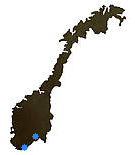
\includegraphics[scale=0.62]{img/norway.png}
    ~
  \section{Languages}
    \asidelist{\textbf{Norwegian}}
    {
\includegraphics[scale=0.30]{img/star.png}
    
\includegraphics[scale=0.30]{img/star.png}
    
\includegraphics[scale=0.30]{img/star.png}
    
\includegraphics[scale=0.30]{img/star.png}
    
\includegraphics[scale=0.30]{img/star.png}}
    \asidelist{\textbf{English}}
    {
\includegraphics[scale=0.30]{img/star.png}
    
\includegraphics[scale=0.30]{img/star.png}
    
\includegraphics[scale=0.30]{img/star.png}
    
\includegraphics[scale=0.30]{img/star.png}
    
\includegraphics[scale=0.30]{img/star_empty.png}}
    \asidelist{\textbf{Faroese}}
    {
\includegraphics[scale=0.30]{img/star.png}
    
\includegraphics[scale=0.30]{img/star.png}
    
\includegraphics[scale=0.30]{img/star_empty.png}
    
\includegraphics[scale=0.30]{img/star_empty.png}
    
\includegraphics[scale=0.30]{img/star_empty.png}}
    \asidelist{\textbf{German}}
    {
\includegraphics[scale=0.30]{img/star.png}
    
\includegraphics[scale=0.30]{img/star_empty.png}
    
\includegraphics[scale=0.30]{img/star_empty.png}
    
\includegraphics[scale=0.30]{img/star_empty.png}
    
\includegraphics[scale=0.30]{img/star_empty.png}}
    ~
\end{aside}



\section{Projects}
\begin{entrylist}
  \entry
    {Oct. 16 - Now}
    {Brobet API \& Android app}
    {Project with Sondre Sallaup}
    {Spare time project with Sondre Sallaup, where I created and maintained
    the backend stack and native Android application.
    Backend stack consisted of a NodeJS (v6.x LTS) TypeScript GraphQL API with
    a PostgreSQL database using the ApolloStack libraries/toolset, ExpressJS http/ws server
    framework and Twitter Digits for authentication.
    \underline{Private repo}.\\}
  \entry
    {Aug. 15 - Oct. 15}
    {UiA Schedule for Android}
    {EnterCon project}
    {An Android application for displaying the schedule is a user-friendly,
    mobile-friendly manner. The scraping-logic from the C\# Schedule Scraper below
    was ported to Java so that the app runs natively.
    \underline{\href{https://github.com/EnterCon/UiA-Timeplan-Android}
    {Github repository}}.\\}
  \entry
    {June 15}
    {UiA Schedule Scraper}
    {Solo project}
    {A C\# console application scraping university programme schedule information
    of their webpage, outputting JSON.
    \underline{\href{https://github.com/EnterCon/UiA-ScheduleScraper}
    {Github repository}}.\\}
\end{entrylist}


\section{Certifications}
\begin{entrylist}
  \entry
    {Oct. 15}
    {PRINCE2 Foundation certification}
    {University of Agder, Kristiansand}
    {Foundation-level Project Management certification.}
\end{entrylist}

\vspace{1.5cm}
\begin{flushright}
\emph{Martin Othamar}
\end{flushright}
\begin{flushright}
\emph{\today}
\end{flushright}

\end{document}
